\documentclass{article} % For LaTeX2e
\usepackage{nips15submit_e,times}
\usepackage[colorlinks,linkcolor=red]{hyperref}
\usepackage{url}
\usepackage{amsmath}
\usepackage{graphicx}
\usepackage{float}
\usepackage{bm}
\usepackage{amssymb}
%\documentstyle[nips14submit_09,times,art10]{article} % For LaTeX 2.09


\title{CS499 Homework 5 (First Draft)}


\author{
	Intersteller\thanks{ Use footnote for providing further information
		about author (webpage, alternative address)---\emph{not} for acknowledging
		funding agencies.}
	Department of Computer Science
	Cranberry-Lemon University
	Pittsburgh, PA 15213
}

% The \author macro works with any number of authors. There are two commands
% used to separate the names and addresses of multiple authors: \And and \AND.
%
% Using \And between authors leaves it to \LaTeX{} to determine where to break
% the lines. Using \AND forces a linebreak at that point. So, if \LaTeX{}
% puts 3 of 4 authors names on the first line, and the last on the second
% line, try using \AND instead of \And before the third author name.

\newcommand{\fix}{\marginpar{FIX}}
\newcommand{\new}{\marginpar{NEW}}

%\nipsfinalcopy % Uncomment for camera-ready version

\begin{document}

	\maketitle
	\textbf{Exercise 5.1}\par

\textbf{(1)} The degree of a vertex is defined as the number of edges linked to this vertex. And the score of a graph is a sequence ranking degree of all vertices from small to big.\par

\textbf{(2)} Graph score theorem states that, if we can find a graph for graph score $(d_1, \cdots ,d_{n-1},d_n)$, then we can find a graph for graph score $(d_1, \cdots ,d_{n-d_n-1},d_{n-d_n}-1,\cdots d_{n-1}-1)$, and vice versa. If we finally get graph score $(\phi)$, the graph exists.\par

\textbf{(3)} Graph score algorithm:\\
First, we get a graph score $(d_1, \cdots ,d_{n-1},d_n)$.\\
If $d_N>n-1$, we cannot find a graph. Otherwise, we add an edge from $d_n$ to $d_{n-d_n},\cdots d_{n-1}$, and check the graph score $(d_1, \cdots ,d_{n-d_n-1},d_{n-d_n}-1,\cdots d_{n-1}-1)$ after it is sorted.\\
We repeat the previous step. If the graph score finally comes to $(\phi)$, the graph exists.\par

\textbf{(4)} The most difficult part is to prove if we can find a graph for graph score $(d_1, \cdots ,d_{n-1},d_n)$, then we can find a graph for graph score $(d_1, \cdots ,d_{n-d_n-1},d_{n-d_n}-1,\cdots d_{n-1}-1)$. We can suppose there is a solution without edge between $n$ and $k$ $(n-d_n\leq k\leq n-1)$, so n must have another link with $j \ (j\leq n-d_{n-1}<k)$. As $j<k$, we know $d_j\leq d_k$, so $k$ must have edge with some point $l$ and $l\neq k$. We change the edges $(n,j)\  (k,l)$ to $(n,k)\  (j,l)$, and we add an edge between $n$ and $k$ without changing the score. In this way, we can transform the answer to make sure there is an edge from $d_n$ to $d_{n-d_n},\cdots ,d_{n-1}$. Then we delete these edges, we get a graph for score $(d_1, \cdots ,d_{n-d_n-1},d_{n-d_n}-1,\cdots d_{n-1}-1)$.\par

\textbf{Exercise 5.8\&5.9}\par
	(Score Theorem for Graphs with Real Edge Weights). Let $(a_1,\cdots, a_n)\in\mathbb{R}^n$. 
	There is a graph with real edge weights with this score if and only if $n=2$ and $a_1=a_2$ or $n\ge 3$.
	 
\textbf{Exercise 5.10}\par
	\textbf{Proof:}
	If $n=2$ and $a_1=a_2$, it is obviously true.\par
	Consider $n\ge 3$, we let the graph be a $n$ polygon. For each edge between adjacent vertexes, the edge weight is $x_i$. 
	Thus we have $(x_1,\cdots, x_n)\in\mathbb{R}^n$ and  $n$ equations:
	\begin{align*}
	x_{n}+x_1&=a_1\\
	x_1+x_2&=a_2\\
	x_2+x_3&=a_3\\
	\cdots\\
	x_{n-1}+x_{n}&=a_{n}
	\end{align*}
	Obviously there are $n$ variables and $n$ equations, so there must exist real solutions for $x_i$.\par
	Thus, for any $(a_1,\cdots, a_n)\in\mathbb{R}^n$ and $n\ge 3$, there must exist a graph with real edge weights with this score.



	\textbf{Exercise 5.11}\par
	(For convenience, we ignore the 0 (a dot) in the following)\par
	\textbf{ID:517030910250}\par
	(1)(2) It is neither a graph score nor a multigtaph score because the sum of the ID is an odd number.
	(3) It is a weighted graph score, as is shown in the following figure.
	
	\begin{figure}[H]
		\centering
		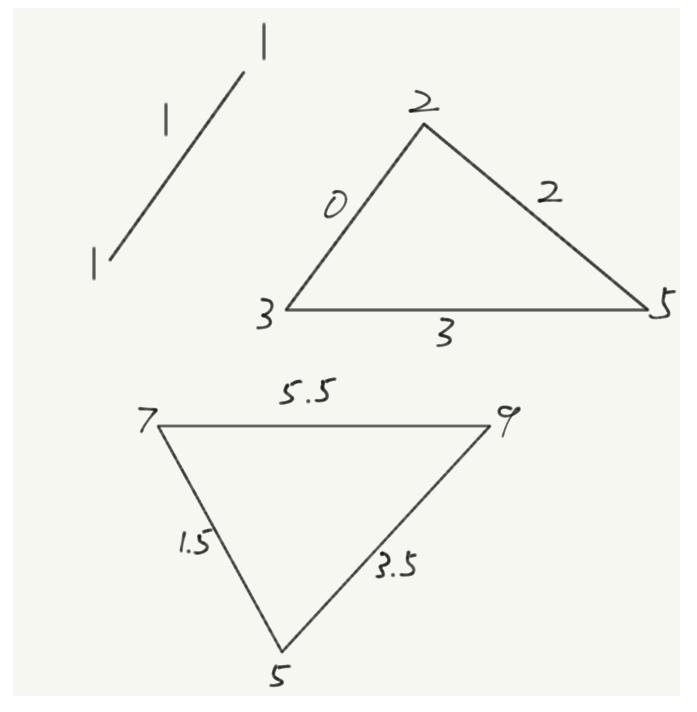
\includegraphics[scale=0.6]{10250.png}
		\caption{}
		\label{fig:1}
	\end{figure}
	(4)Since it is a weighted graph score, it is the score of a graph with real edge weights.

	\textbf{ID:517030910258}\par
	(1)(2) It is neither a graph score nor a multigtaph score because the sum of the ID is an odd number.
	(3) It is a weighted graph score, as is shown in the following figure.
	
	\begin{figure}[H]
		\centering
		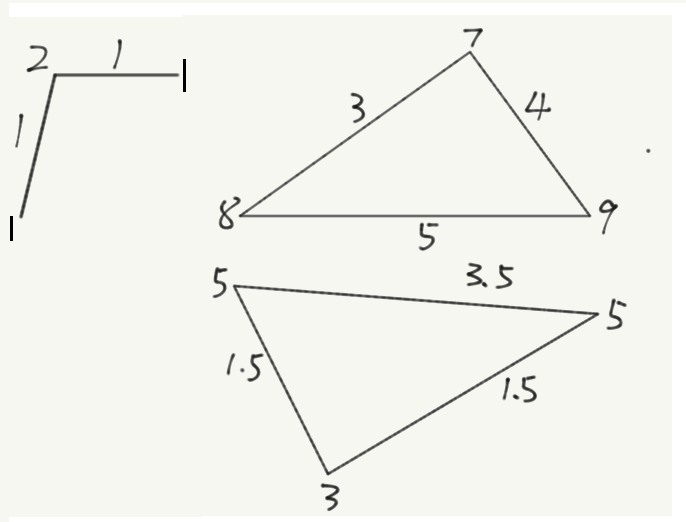
\includegraphics[scale=0.6]{10258.png}
		\caption{}
		\label{fig:2}
	\end{figure}
	(4)Since it is a weighted graph score, it is the score of a graph with real edge weights.

	\textbf{ID:517030910029}\par
	(1)(2) It is neither a graph score nor a multigtaph score because the sum of the ID is an odd number.
	(3) It is a weighted graph score, as is shown in the following figure.
	
	\begin{figure}[H]
		\centering
		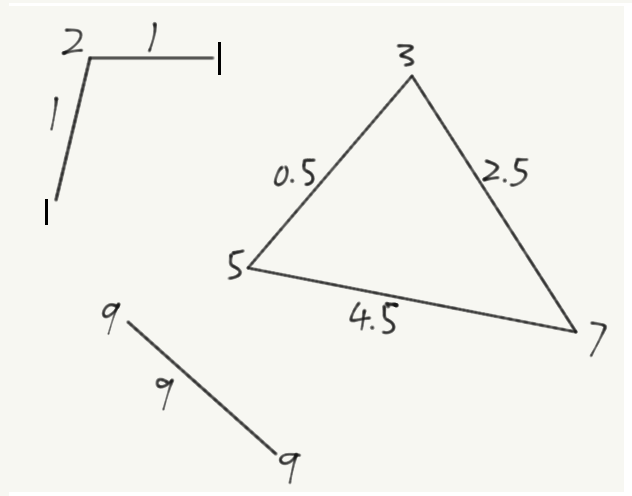
\includegraphics[scale=0.6]{10029.png}
		\caption{}
		\label{fig:3}
	\end{figure}
	(4)Since it is a weighted graph score, it is the score of a graph with real edge weights.

	\textbf{ID:517030910227}\par
	(1)(2) It is neither a graph score nor a multigtaph score because the sum of the ID is an odd number.
	(3) It is a weighted graph score, as is shown in the following figure.
	
	\begin{figure}[H]
		\centering
		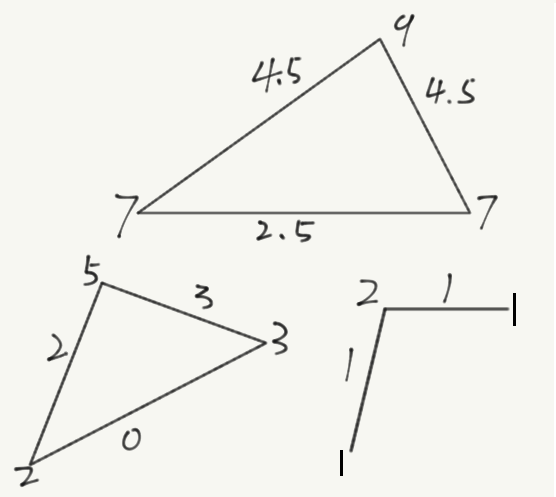
\includegraphics[scale=0.6]{10227.png}
		\caption{}
		\label{fig:4}
	\end{figure}
	(4)Since it is a weighted graph score, it is the score of a graph with real edge weights.

	\textbf{ID:517030910263}\par
	(1)(2) It is neither a graph score nor a multigtaph score because the sum of the ID is an odd number.
	(3) It is a weighted graph score, as is shown in the following figure.
	
	\begin{figure}[H]
		\centering
		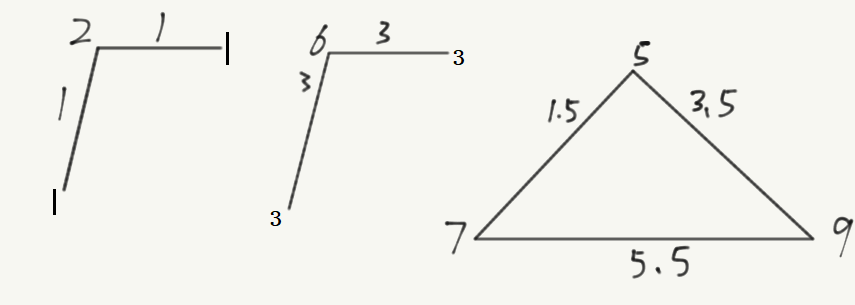
\includegraphics[scale=0.6]{10263.png}
		\caption{}
		\label{fig:5}
	\end{figure}
	(4)Since it is a weighted graph score, it is the score of a graph with real edge weights.

	\textbf{Questions}\par
	


\end{document}
	

